\subsection{Implementering}
\subsubsection{Nodefinder}
\textbf{Problem}\\
Hvordan kan systemme selv gemme alt data i et map.\\
\textbf{Eksemple } \\
Håndtering af input fra aktøren i UI. 
\begin{figure} [hbt!]
\begin{lstlisting}
public ArrayList<Node> getAllNodesFromRoot(Parent root) {
	ArrayList<Node> nodes = new ArrayList<>();
	addAllDescendentsFromNode(root, nodes);
	return nodes;
}
    
private void addAllDescendentsFromNode(Parent parent, ArrayList<Node> nodes){
	for (Node node : parent.getChildrenUnmodifiable()) {
		nodes.add(node);
		if (node instanceof Parent) {
			if (node instanceof TextInputControl) {
				if (!((TextInputControl) node).getText().isEmpty()) {
					String key = node.getId().substring(5);
					nodeMap.put(key, ((TextInputControl) node).getText());
				}
			}
			if (node instanceof RadioButton) {
				if (((Toggle) node).isSelected()) {
					String key = node.getId().substring(5,((RadioButton) node).getId().length() - 1);
					nodeMap.put(key, ((Labeled) node).getText());
				}
			}
			addAllDescendentsFromNode((Parent) node, nodes);
		}
    }
}
\end{lstlisting}
\caption{Data input håndtering}
\label{kode:nodes}
\end{figure}
\textbf{Løsning }\\
”NodeFinder” der har til formål at håndtering input Aktøren. Klassen har ansvaret igennem metoderne ”addAllDescendentsFromNode” og ”getAllNodesFromRoot” at samle alle nodes og gennem værdierne i et ”map” hvor nøglen er node id og værdien er den værdig der ligger i den node. Den har også formålet at sortere node der er i den forældrenode så vi kun kan få de nods der har en betydning den data vi skal has sat ind. \\
”getAllNodesFromRoot” tager alle "nods der ligger på den root node og ligger dem i en ArrayList. ”addAllDescendentsFromNode” tager alle node der er i arraylisten og køre dem igennem. Alle de nodes der er en parent node til en node køres igennem igen for at finde alle de nodes der enten er en ”Textinputcontrole” eller en ”radiobutton” og samler dem i et map.  Dette map bliver samlet med 2 andre maps ” ”cRegardingMap” og ”cRequestingMap” disse 3 maps udgøre til sammen hele sagen.\\
\textbf{Evaluering } \\
\begin{figure} [htb!]
	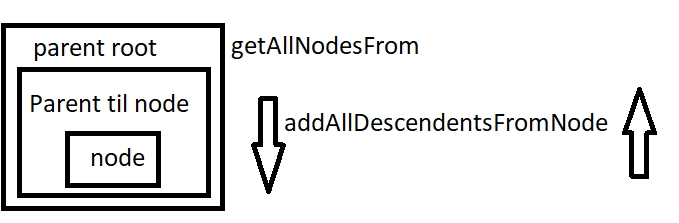
\includegraphics[scale = 0.7]{./PNG/imp/nodes.PNG} 
	\caption{Viser oprationen for hvordan den henter alle nodes}
	\label{fig:nodes}
\end{figure}
”NodeFinder” kan implementeres i alle fxml og samle den specifik data, hvis node id passer med det kolonnen navn i databasen. Dette gør at det bliver nemmer for fremtidige programøre at implementere fxml dokumenter i systemet og samle den data der bliver sat ind.

\subsubsection{Search case}
\textbf{Problem} \\
Hvilke informationer har domænelaget brug for og hvor skal det hentes fra, når der bliver foretaget en søgning?\\
\textbf{Eksempel} \\
Domænelaget sender to værdier til persistens laget. Værdierne skal behandles så "search-Key" bestemmer hvordan der skal søges og værdien "searchValue" hvad der skal søges efter.\\
\textbf{Løsning} \\
Public List search(String searchKey, String searchValue)\\
Der er blevet valgt at ”searchKey” argumentet, håndteres som en af to prædefinerede sætninger: ”case” eller ”citizen”.\\
Argumentet ”searchValue”, består af de attributter som bruges til at finde den ønskede data, samt autorisere personens ret til at se dem.\\
Ved brug af ”case” sætningen, aktiveres en SQL-Query, som leder efter en enkelt sag. Denne Query benytter attributter fra ”searchValue” til at udfylde metodens wildcards:\\
”caseid”(Erstatter de første tre wildcards) og ”departmentid”(Erstatter det fjerde wildcard).\\
Kontrollen af ”departmentid”, bruges til at autorisere et bosteds ansvarsområde i databasen. Hvis brugeren som søger på sagen, arbejder i den afdeling der behandler sagen, vil de kunne se data-outputtet der sendes med ”SearchCase” objektet.\\
Der bruges et ”caseid” til at identificere den specifikke sag der søges. Dette gøres ved hjælp af en Sub-Query, der sorteres efter ”datestamp” blandt de sager som har samme ”caseid”. Denne Sub-Query bruges til at hente de relevante data, fra den seneste udgave af en sag.
\begin{figure} [htb!]
\begin{lstlisting}
if(searchKey.equals("Case")) {
	try {
		connectToDB();
			if(dbConnection != null) {
				String[] search = searchValue.split("%");
				selectQuery = "SELECT c.caseid, c.casestatus, to_char(c.createddate, 'DD/MM-YYYY'),
				ci.citizenid, CONCAT(ci.firstname, ' ', ci.lastname) AS citizenName,
				to_char(cc.datestamp, 'DD/MM-YYYY') AS datestamp, cc.regardinginquiry,
				CONCAT(e.firstname, ' ', e.lastname) AS employeeName, e.employeeid ";
				
				fromQuery = "FROM \"case\" as c, citizen AS ci, (SELECT casecaseid, datestamp,
				regardinginquiry FROM case_contents WHERE casecaseid = ? ORDER BY datestamp DESC LIMIT 1)
				AS cc, (SELECT casecaseid, employeeemployeeid FROM case_employee
				WHERE casecaseid = ?) AS ce, employee AS e ";
				
				whereQuery = "WHERE ce.casecaseid = c.caseid AND e.employeeid = ce.employeeemployeeid 
				AND cc.casecaseid = c.caseid AND ci.citizenid = 
				c.citizenregardingcitizenid AND c.caseid = ? AND
				c.departmentdepartmentid = ? ORDER BY c.caseid DESC;";
				
				query = selectQuery + fromQuery + whereQuery;
				searchCaseStmt = dbConnection.prepareStatement(query);
				searchCaseStmt.setString(1, search[0]);
				searchCaseStmt.setString(2, search[0]);
				searchCaseStmt.setString(3, search[0]);
				searchCaseStmt.setInt(4, Integer.valueOf(search[1]));
				dbResultSet = searchCaseStmt.executeQuery();
				while(dbResultSet.next()) {
					sc.add(new SearchCase(dbResultSet.getInt(4), dbResultSet.getString(5), dbResultSet.
					getString(1), dbResultSet.getString(2), dbResultSet.getString(6),
					dbResultSet.getString(3), dbResultSet.getString(7), 
					dbResultSet.getInt(9), dbResultSet.getString(8)));
                    }
                }
\end{lstlisting}
\end{figure}
\\Ved brug af ”citizen” sætningen, aktiveres en SQL-Query, som søger data på baggrund af en borgers CPR-nummer navn, adresse, gadenummer og/eller postkode.\\
\begin{figure} [htb!]
\begin{lstlisting}
else if(searchKey.equals("Citizen")) {
            try {
                connectToDB();
                if(dbConnection != null) {
                    String[] search = searchValue.split("%");
                    List<String> searchVal = new ArrayList();
                    String searchQuery = "";
                    int columns = 0;
                    if(!search[0].equals("")) {
                        searchQuery += "\"CPR-nr\" LIKE ?";
                        columns++;
                        searchVal.add(search[0]);
                    } 
                    if(!search[1].equals("")) {
                        if(!searchQuery.equals("")) {
                            searchQuery += " AND ";
                        }
                         searchQuery += "CONCAT(ci.firstname, ' ', ci.lastname) LIKE ?";
                         columns++;
                         searchVal.add(search[1]);
                    } 
                    if(!search[2].equals("") || !search[3].equals("")) {
                        if(!searchQuery.equals("")) {
                            searchQuery += " AND ";
                        }
                        searchQuery += "(CONCAT(ci.streetname, ' ', ci.houseno) LIKE ?
                        AND CONCAT(ci.zipcodezipcode, ' ', z.cityname) LIKE ?)";
                        columns++;
                        searchVal.add(search[2]);
                        columns++;
                        searchVal.add(search[3]);
                    }
\end{lstlisting}
\end{figure}
\newpage
Denne Query benytter ”departmentid” til at autorisere søgningen, på samme måde som be-skrevet for første ”searchKey”-eksempel.\\
Attributterne der anvendes fra ”searchValue”, placeres i et String array og derefter samles i en liste. Elementerne fra denne liste, kaldes enekltvis mellem to wildcards (\%). Ved at tilføje disse wildcards på hver side, underrettes den pågældende SQL-Query om at der søges på dele af dataværdier. Når en String fra arrayet skal matches i databasen, vil alle elementer med samme værdi blive hentet, så længe at værdien er case sensitive.
(Se figur \ref{code:wild})\\
\begin{figure}
\begin{lstlisting}
searchCaseStmt = dbConnection.prepareStatement(query);
int index = 1;
for(int i = 1; i <= 3; i++) {
	for (int j = 0; j < columns; j++) {
		searchCaseStmt.setString(index, "%" + searchVal.get(j) + "%");
		index++;
	}
}
searchCaseStmt.setInt(index, Integer.valueOf(search[4]));
dbResultSet = searchCaseStmt.executeQuery();
while(dbResultSet.next()) {
	sc.add(new SearchCase(dbResultSet.getInt(4), dbResultSet.getString(5), 
	dbResultSet.getString(1), dbResultSet.getString(2), dbResultSet.getString(6), 
	dbResultSet.getString(3), dbResultSet.getString(7), dbResultSet.getInt(9), 
	dbResultSet.getString(8)));
s}
\end{lstlisting}
\caption{\% search}
\label{code:wild}
\end{figure}
Når søgefunktionen implementeres på denne måde, er det muligt at returnere en bred søg-ning. En List vil blive fyldt med alle elementer som er relevante i forhold til et givent søgeord.\\
Hvis der bliver søgt efter navnet ”Peter”, vil alle der hedder ”Peter” blive hentet. På grund af brugen af wildcards, vil navne hvor ”Peter” indgår i også blive hentet, f.eks:\\
”Anders Petersen”, ”Jens Peter”, ”Peter Halfdan”\\